\documentclass{scrartcl}
\KOMAoptions{
    fontsize=12pt,
    paper=letter,
    paper=portrait,
    parskip=half,
    headings=big,
    toc=listof,
    twoside=false,
	DIV=14,
    }

\usepackage{amsmath, amsthm, amsfonts, graphicx, enumitem, hyperref}

\pagestyle{empty}

\theoremstyle{definition}
\newtheorem{prob}{Problem}

\begin{document}
	\noindent\begin{minipage}{.5\textwidth}{}
		\textsc{Haverford Problem Solving Group}

		\textsc{November 23, 2021}
	\end{minipage}\hfill
	\begin{minipage}{.4\textwidth}{}
		\ \hfill
		
\includegraphics[height = .9in]{psg_logo}
	\end{minipage}\\[.5em]
	\hrule

	\setcounter{prob}{5}
	\begin{prob}
		Can the portion of any parabola inside a circle of radius \(1\) have a length greater than \(4\)?
	\end{prob}

	\setcounter{prob}{9}

	\begin{minipage}{.8\textwidth}{}
		\begin{prob}%[Pick's Theorem]
			Suppose that a polygon has integer coordinates for all of its vertices. Let \(i\) be the number of integer points that are interior to the polygon, and let \(b\) be the number of integer points on its boundary (including vertices as well as points along the sides of the polygon). Then the area of this polygon is \[
				i + \frac{b}{2} - 1.
			\]
		\end{prob}
	\end{minipage}
	\begin{minipage}{.17\textwidth}{}
		\ \hfill
		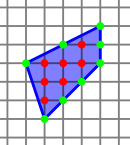
\includegraphics[width=.9\textwidth]{pick}
	\end{minipage}

	\begin{prob}%[Romanian Masters of Mathematics 2018, 2]
		Determine whether there exist non-constant polynomials $P\left(x\right)$ and $Q\left(x\right)$ with real coefficients satisfying \[P\left(x\right)^{10}+P\left(x\right)^9=Q\left(x\right)^{21}+Q\left(x\right)^{20}.\]
	\end{prob}

	\begin{prob}%[Romanian Masters of Mathematics 2018, 3]
		Ann and Bob play a game on an infinite checkered plane making moves in turn. A move consists in orienting any unit grid-segment that has not been oriented before. If at some stage some oriented segments form an oriented cycle, Bob wins.
		\begin{enumerate}[label = (\alph*)]
			\item Bob makes the first move. Does Bob have a strategy that guarantees him to win?
			\item Ann makes the first move. Does Bob have a strategy that guarantees him to win?
		\end{enumerate}
	\end{prob}

	\setcounter{prob}{15}
	\begin{prob}%[Putnam 2011, A3]
		Find a real number $c$ and a positive number $L$ for which
		\[\lim_{r\to\infty}\frac{r^c\int_0^{\pi/2}x^r\sin x\,dx}{\int_0^{\pi/2}x^r\cos x\,dx}=L.\]
	\end{prob}

	\setcounter{prob}{17}
	\begin{prob}%[Putnam 2011, B2]
		Let $S$ be the set of all ordered triples $(p,q,r)$ of prime numbers for which at least one rational number $x$ satisfies $px^2+qx+r=0.$ Which primes appear in seven or more elements of $S?$
	\end{prob}

	\setcounter{prob}{18}
	\begin{prob}
	Let $f:[-1,1]\to\mathbb{R}$ be a continuous function such that:
	\begin{enumerate}[label = \textbullet, itemsep = -.25em]
		\item $f(x)=\frac{2-x^2}{2}f\left(\frac{x^2}{2-x^2}\right)$ for every $x$ in $[-1,1],$
		\item $ f(0)=1,$ and
		\item $\lim_{x\to 1^-}\frac{f(x)}{\sqrt{1-x}}$ exists and is finite.
	\end{enumerate}

	Prove that $f$ is unique, and express $f(x)$ in closed form.
	\end{prob}

	\newpage

	\begin{center}
		\textsc{Previous problems solved by some of us.}
	\end{center}

	\setcounter{prob}{2}
	\begin{prob}
		Find the $2000$\textsuperscript{th} digit in the square root of $N = 11\dots1$, where $N$ contains $1998$ digits, all of them $1$'s.
	\end{prob}

	\setcounter{prob}{13}
	\begin{prob}%[Putnam 2014, B2]
		Suppose that $f$ is a function on the interval $[1,3]$ such that $-1\le f(x)\le 1$ for all $x$ and $\displaystyle \int_1^3f(x)\,dx=0.$ How large can $\displaystyle\int_1^3\frac{f(x)}x\,dx$ be?
	\end{prob}

	\setcounter{prob}{14}
	\begin{prob}%[Putnam 2014, A3]
		Let $a_0=5/2$ and $a_k=a_{k-1}^2-2$ for $k\ge 1.$ Compute \[\prod_{k=0}^{\infty}\left(1-\frac1{a_k}\right)\] in closed form.
	\end{prob}

	\setcounter{prob}{16}
	\begin{prob}%[IMO 1995, 6]
		Let $p$ be an odd prime number. Determine how many $p$-element subsets $A$ of $ \{1,2,\dots,2p\}$ are such that the sum of elements of \(A\) is divisible by $p$.
	\end{prob}


	\vfill

	\begin{minipage}{.85\textwidth}{}
		\footnotesize
		If you are not in our Discord server, you should definitely join.
		We will post there handouts, resources, solutions, room/time changes, and (most important of all) pictures whatever food we will have in the meeting. Point your phone camera to the QR code to join it.
	\end{minipage}
	\begin{minipage}{.15\textwidth}{}
		\ \hfill 
\includegraphics[height = .8in]{qr}
	\end{minipage}
\end{document}
